\chapter{Airfoils Tab}
\label{chap:profils}

The \menu{Airfoils} tab is the heart of the application: it allows
loading, visualizing, editing and comparing airfoils. At startup,
the current airfoil (blue) is a \textbf{NACA~2412} automatically
\textbf{converted to Bézier}, and the reference airfoil (red) is a
\textbf{NACA~2412} in discrete-points mode. By default, the
\textbf{curvature} of the current airfoil, the \textbf{deviation}
between the two airfoils and the \textbf{flap} (deflected at
$-10^\circ$) are also displayed.

\screenshot{02_tab_profils_default.png}{1.0}{%
    \menu{Airfoils} tab in its default state: current airfoil
    (blue, Bézier) with its control points, curvature at the leading
    edge, airfoil with flap (green) and deviation relative to the
    reference.}

\section{Control bar}

The bar located below the tab selector groups the display options,
organized in \textbf{four frames} according to whether they concern
a single airfoil, both, or none.

\subsubsection*{\og Current airfoil \fg{} frame}

\begin{itemize}
    \item \textbf{Current airfoil} (check box): shows or hides the
        current airfoil. The colored label indicates its name (by
        default \og NACA~2412 \fg{}).
    \item \textbf{Curvature}: displays the curvature
        \emph{porcupines} of the current airfoil (segments
        perpendicular to the curve, length proportional to the local
        curvature).
    \item \textbf{Pts}: displays the points actually sampled on the
        splines (markers).
\end{itemize}

\subsubsection*{\og Reference airfoil \fg{} frame}

\begin{itemize}
    \item \textbf{Reference airfoil} and \textbf{Curvature}:
        same for the reference airfoil.
\end{itemize}

\subsubsection*{Global frame (two airfoils / none)}

\begin{itemize}
    \item \textbf{Deviation}: plots the geometric differences
        between current airfoil and reference. The computation
        \textbf{mode} (vertical or normal) is chosen in the
        \menu{Options $\rightarrow$ Deviation} menu. See
        section~\ref{sec:deviation}, page~\pageref{sec:deviation}.
    \item \textbf{Image}: shows or hides the \textbf{tracing image}
        (background) when an image has been loaded. The box remains
        inactive (greyed out) as long as no image is loaded. See
        section~\ref{sec:calque}, page~\pageref{sec:calque}.
\end{itemize}

\subsubsection*{\og Flap \fg{} frame}

\begin{itemize}
    \item \textbf{Flap} (check box): activates the generation and
        display of an airfoil with deflected flap (green).
    \item \textbf{Xf}: position of the hinge axis, in percent of
        chord from the leading edge.
    \item \textbf{Deflection}: flap deflection angle, in degrees
        (positive = trailing edge upward).
\end{itemize}

The flap module is detailed in section~\ref{sec:flap},
page~\pageref{sec:flap}.

\begin{important}
The \textbf{Curvature} options only work on airfoils in
\textbf{spline mode}. If you try to activate them on an airfoil in
discrete-points mode, a warning message is displayed and the box
unchecks itself automatically (see \figref{08_msg_courbure.png}).
\end{important}

\section{Airfoil visualization}

\subsection{Discrete-points mode}

This is the default mode at loading. The airfoil is plotted as a
smooth curve interpolated between the discrete points. No control
point is visible.

\subsection{Spline mode}

Once the airfoil is converted to a spline (see
section~\ref{sec:convertspline}), numerous elements appear:

\screenshot{03_tab_profils_spline.png}{1.0}{%
    Airfoil in spline mode: the blue squares are the interior
    control points of the Béziers; the points surrounded by a circle
    mark the joins between consecutive segments.}

\begin{itemize}
    \item \textbf{Blue squares}: interior control points of the
        Bézier curves. They are \textbf{draggable} with the mouse to
        modify the airfoil shape.
    \item \textbf{Circles with a central point}: join points between
        two consecutive Bézier segments. They are also draggable;
        their movement preserves C\textsuperscript{1} continuity with
        the neighboring segments.
    \item \textbf{Control polygon} (grey dotted lines): connects the
        control points in order.
    \item \textbf{Mean line} (light blue dashes): plots the relative
        camber of the airfoil (average of upper/lower surface).
\end{itemize}

\subsection{Curvature display}

Activating the \textbf{Curvature} box reveals the
\emph{porcupines}: segments perpendicular to the curve, whose length
is proportional to the signed local curvature.

\screenshot{04_tab_profils_courbure.png}{1.0}{%
    Display of the curvature porcupines (orange segments).}

\begin{noteinfo}
Curvature is the inverse of the radius of the osculating circle.
A positive curvature signals a curve concave toward increasing
$y$ (top of the upper surface), negative concave toward decreasing
$y$. Curvature discontinuities are often visible at segment joins
with C1 but not C2 continuity.
\end{noteinfo}

The \textbf{porcupine scale} and their \textbf{density} (number of
quills per curve) are adjustable via the context menu (right-click
on the canvas).

\subsection{Display of sampled points}

The \textbf{Pts} option reveals markers at the positions of the
points actually used for discrete sampling. This is useful to check
the density and distribution of the sampling before export or
simulation.

\screenshot{05_tab_profils_pts.png}{1.0}{%
    Display of the sampling points. The \emph{curvilinear} mode
    (default) distributes the points uniformly along the arc.}

\subsection{Deviation visualization}
\label{sec:deviation}

The \textbf{Deviation} option measures the geometric difference
between the current airfoil and the reference airfoil, as a bundle
of segments (\emph{quills}) accompanied by an envelope. The maximum
deviation is highlighted.

\subsubsection*{Computation modes}

The mode is chosen in the \menu{Options $\rightarrow$ Deviation}
menu:

\begin{itemize}
    \item \textbf{Vertical (thickness)}: the difference is measured
        \textbf{vertically} (along the $z$ axis), at constant
        abscissa $x$, by interpolation of the two airfoils on a
        common grid. This is the default mode, suited to thickness
        comparison.
    \item \textbf{Normal (perpendicular)}: the difference is measured
        \textbf{perpendicular to the surface} of the current airfoil
        (distance along the normal). This mode better reflects the
        actual geometric difference between two curves, in particular
        near the leading edge where the surfaces are strongly
        inclined.
\end{itemize}

\begin{figure}[H]
    \centering
    \fbox{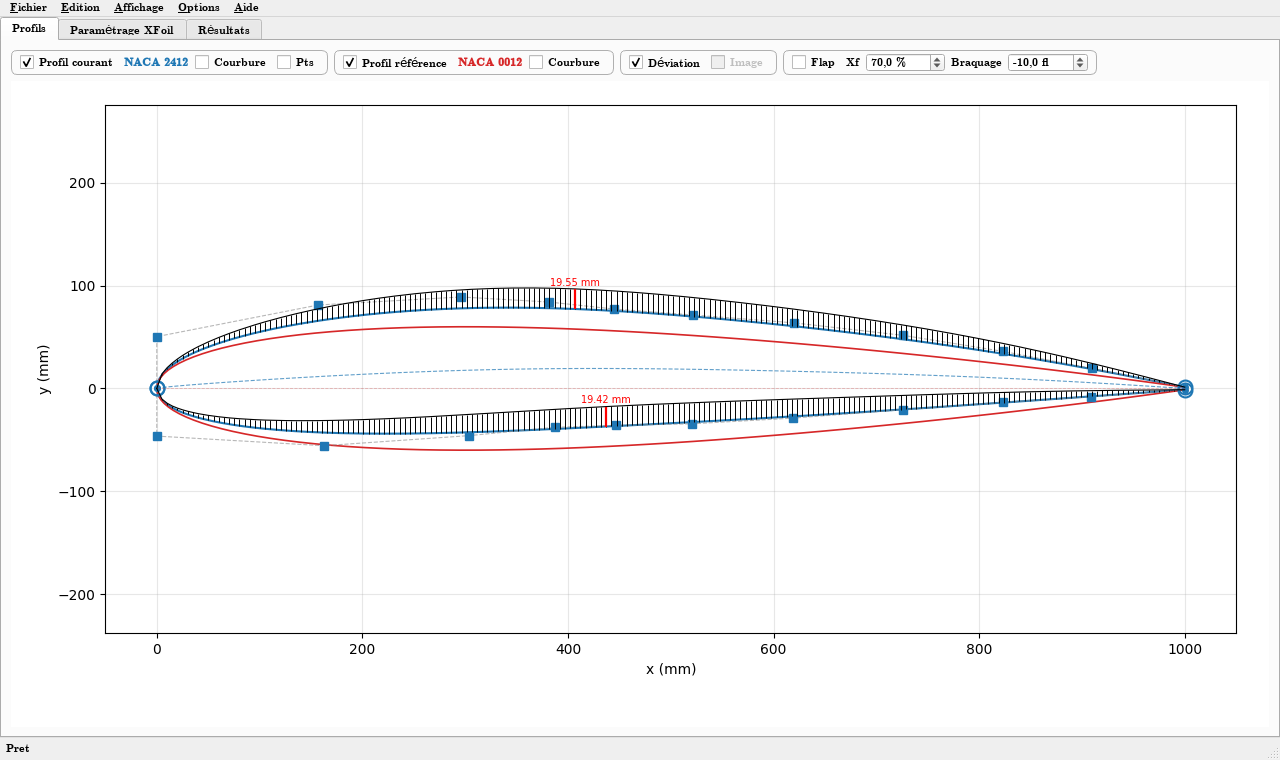
\includegraphics[width=0.49\textwidth]{images/06_tab_profils_deviation.png}}
    \hfill
    \fbox{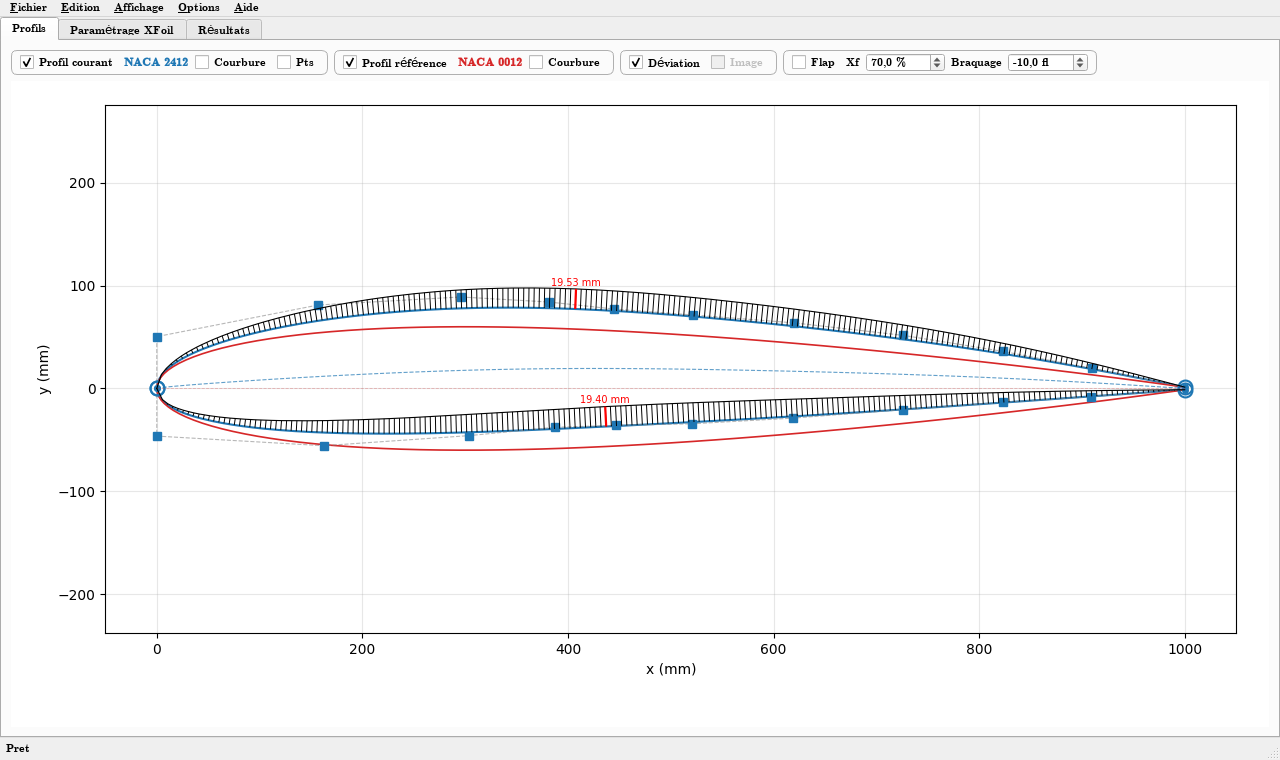
\includegraphics[width=0.49\textwidth]{images/14_deviation_normale.png}}
    \caption{Deviation between NACA~2412 (current, blue) and NACA~0012
        (reference, red). On the left the \emph{vertical} mode
        (vertical quills), on the right the \emph{normal} mode
        (quills perpendicular to the surface). In both cases,
        the maximum-deviation quill is plotted in \textcolor{red}{red}
        with its value in millimeters.}
    \label{fig:06_tab_profils_deviation.png}
\end{figure}

\subsubsection*{Maximum deviation}

The \textbf{maximum} deviation is signaled by a
\textcolor{red}{\textbf{red}} quill bearing its \textbf{value in
millimeters} at its end. The computation is performed:

\begin{itemize}
    \item \textbf{per Bézier segment} if the current airfoil is in
        spline mode (one maximum per upper-surface and lower-surface
        segment);
    \item \textbf{per side} (upper surface, lower surface) if the
        current airfoil is in discrete-points mode.
\end{itemize}

The displayed value is the \textbf{actual} deviation (not
exaggerated), expressed in the unit of the airfoil (millimeters for a
chord of 1\,000~mm).

\begin{astuce}
When the airfoils have a very small deviation to the eye
(for example during an optimization by small displacements of the
control points), it is useful to \textbf{amplify} the deviation
display. The scale is adjustable via the context menu:
\menu{Deviation scale\dots}. This scale only affects the visual
length of the quills, not the value in millimeters displayed at the
maximum.
\end{astuce}

\section{Loading an airfoil from the UIUC database}
\label{sec:uiuc}

AirfoilTools provides \textbf{direct access} to the airfoil database
of the University of Illinois (the \textbf{Selig} collection,
about 1\,600 airfoils), accessible via the entries
\menu{File $\rightarrow$ From the UIUC database $\rightarrow$ Current
airfoil\dots} and \menu{\dots Reference airfoil\dots}.

\screenshot{11_dialog_uiuc.png}{0.7}{%
    Loading dialog from the UIUC database. The search
    \og naca \fg{} filters 183~airfoils out of 1\,613. The selected
    airfoil shows its description below the list.}

\subsection{Usage}

\begin{enumerate}
    \item On the first call, the complete index (~1\,600 airfoils) is
        downloaded from the UIUC server. The download takes a few
        seconds depending on the connection.
    \item Type all or part of the name or description of the airfoil
        in the \menu{Search} field: the list filters in real time
        (case insensitive).
    \item Click on an airfoil to see its description below the list.
        Double-click or the \bouton{Load} button to download and open
        it.
    \item The airfoil is loaded in \textbf{discrete-points mode}
        (Selig format). To benefit from interactive editing, then use
        \menu{Edit $\rightarrow$ Convert to Spline} (see next
        section).
\end{enumerate}

\subsection{Local cache}

To avoid unnecessarily overloading the UIUC server and to allow
offline use:

\begin{itemize}
    \item The \textbf{index} (airfoil list + descriptions) is cached
        for \textbf{7~days}. Beyond that, it is re-downloaded
        automatically.
    \item The downloaded \textbf{\chemin{.dat} files} are cached
        \textbf{permanently} (UIUC airfoils are stable over time).
\end{itemize}

The \bouton{Refresh} button forces the re-download of the index to
retrieve any new airfoils.

The cache location is:

\begin{itemize}
    \item Windows: \chemin{C:\textbackslash{}Users\textbackslash{}<user>\textbackslash{}.airfoiltools\textbackslash{}cache\textbackslash{}uiuc\textbackslash{}}
    \item Linux / macOS: \chemin{\textasciitilde/.airfoiltools/cache/uiuc/}
\end{itemize}

\begin{noteinfo}
The \chemin{.dat} files of the UIUC database follow the
Selig convention (path TE $\rightarrow$ upper surface $\rightarrow$
LE $\rightarrow$ lower surface $\rightarrow$ TE) with a header
line containing the airfoil name. They are directly
usable by AirfoilTools.
\end{noteinfo}

\begin{attention}
An internet connection is required for the first download of the
index and of each airfoil. In case of unavailability of the UIUC
server, the dialog displays an error message; the airfoils already
cached, however, remain usable.
\end{attention}

\section{Generating a NACA airfoil}
\label{sec:naca}

AirfoilTools can generate on the fly the airfoils of the
\textbf{NACA} family from their designation, without going through a
file. Generation is accessible via \menu{File $\rightarrow$ NACA
airfoil $\rightarrow$ Current airfoil\dots} (or
\menu{\dots Reference airfoil\dots}).

\screenshot{16_dialog_naca.png}{0.55}{%
    Entry of the NACA digits. A second dialog then asks for the
    number of points of the airfoil.}

\subsection{Usage}

\begin{enumerate}
    \item Enter the \textbf{digits} in the first dialog:
        \begin{itemize}
            \item \textbf{4 digits} (e.g. \texttt{2412}): maximum
                camber (\%), position of max camber (tenths of
                chord), relative thickness (\%);
            \item \textbf{5 digits} (e.g. \texttt{23012}): cambered
                airfoil with a more complex mean line.
        \end{itemize}
    \item Enter the \textbf{number of points} in the second dialog
        (default 150).
    \item The airfoil is generated, normalized (chord 1\,000~mm) and
        assigned to the chosen role (current or reference).
\end{enumerate}

\subsection{Clean regeneration from the context menu}

An airfoil generated by this function is \textbf{marked} as a NACA
airfoil as long as it has not been modified (editing of a control
point) nor converted to a spline. For such a NACA airfoil in
discrete-points mode, the \textbf{context menu} (right-click) offers
the entry \menu{Number of points\dots}.

Changing the number of points this way does not merely interpolate
the existing points: it \textbf{recalls the NACA generation
function} to produce a \emph{clean} airfoil at the new resolution,
conforming to the analytical formula.

\begin{noteinfo}
This clean regeneration is only possible for an \textbf{unmodified}
NACA airfoil. As soon as it is converted to a spline or edited,
the marker is lost: one then reverts to the classic
re-sampling of the spline.
\end{noteinfo}

\section{Conversion to spline}
\label{sec:convertspline}

To benefit from interactive editing, the airfoil must be converted
to spline mode. This is done via:

\begin{itemize}
    \item the \menu{Edit $\rightarrow$ Convert to Spline} menu;
    \item the keyboard shortcut \touche{Ctrl}+\touche{B}.
\end{itemize}

A dialog opens to enter the conversion parameters:

\screenshot{07_dialog_convert.png}{0.45}{%
    Conversion-to-spline dialog.}

\begin{tabularx}{\linewidth}{l X}
    \toprule
    \textbf{Parameter} & \textbf{Description} \\
    \midrule
    Upper-surface degree
        & Degree of the Bézier curves of the upper surface.
          Small (3--5) = very smoothed shape; medium (6--12) =
          compromise (recommended); large ($>$~15) = very precise
          shape but risk of oscillations.\\
    Lower-surface degree
        & Same for the lower surface. Can differ from the
          upper-surface degree (typically the lower surface is less
          curved).\\
    Tolerance
        & Maximum deviation accepted between the fitted spline and
          the discrete points, as a fraction of the chord.
          Typical value: $10^{-3}$ to $10^{-4}$.\\
    Max segments
        & Maximum number of Bézier segments per side.
          With 1, a single global segment is obtained (historical
          behavior). With a higher value and a fine tolerance, the
          \emph{adaptive} algorithm splits at the point of greatest
          error until the tolerance is met, concentrating the
          segments in zones of high curvature (typically the leading
          edge).\\
    Smoothing
        & Regularization coefficient of the fit (Tikhonov).
          $0$ = pure least-squares fit; $>0$ = smoothing of the
          control polygon.\\
    \bottomrule
\end{tabularx}

\begin{astuce}
For most airfoils, parameters of \textbf{degree 11},
\textbf{tolerance $10^{-3}$}, \textbf{max segments 4},
\textbf{smoothing 0{,}1} give a good compromise between precision
and geometric quality. Reduce the tolerance to $10^{-4}$ and
increase \emph{Max segments} to 8--10 for a very faithful
approximation.
\end{astuce}

\section{Interactive editing}

In spline mode, the canvas becomes an \textbf{interactive geometric
editor}.

\subsection{Mouse interactions}

\begin{tabularx}{\linewidth}{l X}
    \toprule
    \textbf{Action} & \textbf{Effect} \\
    \midrule
    Left click + drag on a control point
        & Moves the control point. The curve is updated in real
          time.\\
    Left click + drag in empty space
        & Draws a \emph{zoom rectangle}. The view is reframed on the
          zone at the end of the drag.\\
    Mouse wheel
        & Zoom centered on the cursor position.\\
    Middle click (or \touche{Shift}+left click)
        & Pan (translation of the view).\\
    Right click
        & Opens the \textbf{context menu}.\\
    \bottomrule
\end{tabularx}

\subsection{Context menu (right-click)}

The context menu offers several actions depending on the context:

\begin{itemize}
    \item \menu{Point info\dots} (if clicking on a control point):
        displays the coordinates and local parameters of the point.
    \item \menu{Release the vertical tangency constraint at the
        leading edge} (if clicking on the P1 node, neighbor of the
        leading edge): releases or restores the vertical tangent at
        the leading edge. See section~\ref{sec:batangente}.
    \item \menu{Porcupine scale\dots}: sets the display scale of the
        curvature.
    \item \menu{Porcupine density / $\times 2$ or $\div 2$}:
        modifies the number of quills displayed.
    \item \menu{Deviation scale\dots} and \menu{Deviation density}:
        same for the deviation porcupines.
    \item \menu{Split upper surface / Split lower surface} (in spline
        mode): splits the spline in two at the nearest clicked point
        (De Casteljau algorithm, exact).
    \item \menu{Global parameters}: number of sampling points,
        method (curvilinear or adaptive).
    \item \menu{Segment} (if clicking within a specific segment):
        allows defining \emph{per-segment overrides} (degree, number
        of points, method different from the global one).
\end{itemize}

\subsection{Vertical tangent at the leading edge}
\label{sec:batangente}

By default, the first interior control point of each side
(noted \textbf{P1}, neighbor of the leading edge) is
\textbf{constrained} to remain on the vertical of the leading edge
(LE). This constraint guarantees a \textbf{vertical tangent} at the
leading edge, which corresponds to the natural geometry of most
airfoils. During editing, the movement of P1 is therefore limited to
the vertical axis.

\screenshot{13_ba_tangente.png}{1.0}{%
    Effect of the vertical-tangent constraint at the leading edge.
    On the left, constraint active: the P1 node (circled in red)
    stays aligned vertically with the LE, the tangent (red dashes) is
    vertical. On the right, constraint released: P1 can be moved
    freely, the tangent tilts.}

It is sometimes desirable to \textbf{release} this constraint (for
example to trace an airfoil whose leading edge does not have a
strictly vertical tangent). To do so:

\begin{enumerate}
    \item Perform a \textbf{right-click} on the P1 node of the
        upper surface or lower surface.
    \item Choose \menu{Release the vertical tangency constraint at
        the leading edge}.
\end{enumerate}

The P1 node then becomes freely draggable (in $x$ and $y$). To
restore the constraint, right-click again on the node and choose
\menu{Restore the vertical tangency at the leading edge}: the P1
node is automatically brought back onto the vertical of the leading
edge.

\begin{noteinfo}
The constraint is managed \textbf{independently} for the upper
surface and the lower surface. Releasing the tangent on the
upper-surface side does not affect the lower surface, and vice
versa.
\end{noteinfo}

\section{Flap}
\label{sec:flap}

The \textbf{flap} module generates a \textbf{deflected airfoil} from
the current airfoil, by rotating its rear part around a hinge axis.
The airfoil with flap is plotted in \textbf{green}, in addition to
the current and reference airfoils; it is \textbf{not editable}
(recomputed automatically) and can be simulated then saved like the
current airfoil.

\screenshot{15_tab_profils_flap.png}{1.0}{%
    Airfoil with flap (green) deflected at $-10^\circ$ at 70~\% of
    chord, superimposed on the current airfoil (blue) and its
    control points.}

\subsection{Activation and settings}

The controls are in the \og Flap \fg{} frame of the \menu{Airfoils}
tab bar:

\begin{tabularx}{\linewidth}{l X}
    \toprule
    \textbf{Control} & \textbf{Role} \\
    \midrule
    \textbf{Flap} & Activates the generation of the deflected airfoil (green). \\
    \textbf{Xf} & Position of the hinge axis, in \textbf{percent of
        chord} measured from the leading edge (5 to 95~\%). \\
    \textbf{Deflection} & Deflection angle in degrees ($-45$ to
        $+45$). \textbf{Positive} = trailing edge \textbf{upward};
        \textbf{negative} = trailing edge \textbf{downward}. \\
    \bottomrule
\end{tabularx}

The deflected airfoil is recomputed in real time at each change of
\menu{Xf} or \menu{Deflection}, and at each modification of the
current airfoil.

\subsection{Hinge geometry}

The hinge axis is the \textbf{center of the inscribed circle}
tangent simultaneously to the upper surface and the lower surface,
whose abscissa equals \menu{Xf}. The rear part of each surface is
then rotated by the deflection angle around this axis.

\screenshot{19_flap_schema.png}{0.95}{%
    Construction of the hinge: the inscribed circle (green),
    tangent to the upper surface and the lower surface at the
    abscissa $X_f$, provides the rotation center (red point) of the
    flap.}

Depending on the side and the sign of the deflection, the join
between the fixed part and the deflected part is handled
differently:

\begin{itemize}
    \item on the side where the deflection \textbf{opens} a gap, an
        \textbf{arc of circle} fills the space;
    \item on the side where the deflection \textbf{closes back} the
        material, the surface is \textbf{cut at the intersection}
        (overlap removed).
\end{itemize}

\subsection{Simulation and saving}

\begin{itemize}
    \item \textbf{Simulation}: the airfoil with flap is simulated by
        XFoil in the same way as the current and reference airfoils.
        The \bouton{Flap only} button of the \menu{XFoil Settings}
        tab computes it in isolation; \bouton{Run all} includes it if
        it is active. The results appear under the \emph{Flap} role
        (green) in the \menu{Results} tab.
    \item \textbf{Saving}: \menu{File $\rightarrow$
        Save airfoil with flap\dots} saves the deflected airfoil,
        with the same complete / upper-surface / lower-surface choice
        and the same formats as the current airfoil.
\end{itemize}

\begin{important}
For the simulation, the airfoil with flap is expressed in the
\textbf{normalized frame of the current airfoil}: XFoil neither
re-normalizes nor re-aligns it. One thus observes only the effect of
the deflection relative to the current airfoil (shift of the polar,
of the moment, etc.), without any artifact of change of chord or of
reference angle of attack.
\end{important}

\section{Tracing image (tracing an airfoil)}
\label{sec:calque}

AirfoilTools allows loading a \textbf{background image} (photo, scan
of a drawing, screenshot of an airfoil) in order to \textbf{trace}
its shape by moving the control points of the current airfoil until
they match the silhouette of the image.

\screenshot{12_tab_profils_calque.png}{1.0}{%
    Tracing an airfoil: the tracing image (grey silhouette) is
    displayed in the background; the current airfoil (blue, in spline
    mode) and its control points are superimposed on top. The control
    points are adjusted to make the blue curve coincide with the
    silhouette.}

\subsection{Loading the image}

Loading is done via \menu{File $\rightarrow$ Load tracing
image\dots}. The usual formats are accepted: \chemin{.jpg},
\chemin{.png}, \chemin{.tif}, \chemin{.bmp}. On opening, the image
is scaled to cover approximately the chord (1\,000~mm) and the
\textbf{Image} box of the control bar becomes active and checked.

The image is drawn \textbf{in the background}, beneath the airfoil
and its control points, which therefore remain perfectly visible and
manipulable on top.

\subsection{Positioning, scaling and rotating the image}

The manipulations of the image are done by holding the
\touche{i} key down, combined with the mouse:

\begin{tabularx}{\linewidth}{l X}
    \toprule
    \textbf{Action} & \textbf{Effect} \\
    \midrule
    \touche{i} + left click dragged
        & \textbf{Moves} the image (translation).\\
    \touche{i} + mouse wheel
        & \textbf{Scales} the image (enlarges / reduces around its
          center).\\
    \touche{i} + right click dragged
        & \textbf{Rotates} the image around the origin $(0,0)$
          (the leading edge).\\
    \touche{Shift} + \touche{i} + action
        & \textbf{Fine adjustments}: movement and rotation ten times
          slower, reduced scaling step. Ideal for precise
          alignment.\\
    \bottomrule
\end{tabularx}

\begin{astuce}
Proceed in two steps: first a coarse alignment (movement,
scaling, rotation without \touche{Shift}) to superimpose the image
and the airfoil approximately, then a \textbf{fine adjustment}
holding \touche{Shift} for the precise alignment of the leading edge
and the trailing edge.
\end{astuce}

\begin{noteinfo}
The canvas must have the \textbf{keyboard focus} for the
\touche{i} key to be taken into account: it obtains it automatically
as soon as the cursor hovers over the plotting area.
\end{noteinfo}

\subsection{Hiding or removing the image}

\begin{itemize}
    \item The \textbf{Image} box of the control bar shows or hides
        the image without deleting it.
    \item \menu{File $\rightarrow$ Remove the tracing image}
        permanently removes the image from the session.
\end{itemize}

\begin{important}
The tracing image and its position (scale, rotation, translation)
are \textbf{saved with the project} in the \chemin{.aftproj} format
(see chapter~\ref{chap:formats}). One thus finds the tracing exactly
as it was upon reopening the project. The classic airfoil formats
(\chemin{.dat}, \chemin{.bspl}\dots) do \textbf{not} contain the
image: to keep the tracing, a project must be saved.
\end{important}

\section{\og Curvature unavailable \fg{} warning}

When the \menu{Curvature} box is activated while the concerned
airfoil is in discrete-points mode (not converted to spline),
an information message is displayed:

\screenshot{08_msg_courbure.png}{0.7}{%
    \og Curvature unavailable \fg{} warning message.}

As indicated in the message, two solutions are possible:

\begin{enumerate}
    \item convert the airfoil to a spline (menu
        \menu{Edit $\rightarrow$ Convert to Spline});
    \item load an airfoil in a format preserving the spline geometry
        (\chemin{.bspl} or \chemin{.bez}).
\end{enumerate}

The box unchecks itself automatically after the message is
displayed.

\section{Modifying the number of points}

In spline mode, the number of discrete sampling points of the
splines can be modified via the \menu{Edit $\rightarrow$
Sampling $\rightarrow$ Current airfoil\dots} menu (or
\menu{\dots Reference airfoil\dots}).

A dialog asks for the new number of points (between 10 and
10\,000). This affects only the \emph{export discretization} and the
display: the underlying spline geometry is not altered.

\begin{noteinfo}
For XFoil simulations, the default sampling
(150~points) is generally sufficient. XFoil then re-samples
internally via the \texttt{PANE} command if the \emph{Repanel}
option is activated in the \menu{XFoil Settings} tab.
\end{noteinfo}
